\chapter{Conclusione}

\section{Analisi delle performance}

\subsection{Limiti dell'applicazione}

\subsubsection{Limiti imposti da MediaPipe}
\begin{enumerate}
    \item \textbf{Framerate limitato}: comprensibile contando che siamo su dispositivi mobile, meno elaborazioni facciamo meno batteria viene consumata.
    \item \textbf{Dati imprecisi quando non tutte le dita vengono mostrate}: se si mostra una gesture che non espone tutte le dita bene in vista (pollice in su) e si muove la mano cambiando punto di vista, le coordinate rilevate dalla libreria non rimangono coerenti.
    \item \textbf{Applicazione basata su immagini ben illuminate}: se nello stream video manca di luminosità l'accuratezza del rilevamento cala drasticamente (problema noto nel mondo di computer vision)
\end{enumerate}

\subsubsection{Limiti della nostra soluzione}
\begin{enumerate}
    \item \textbf{Consumo batteria relativamente elevato}: per una app mobile porre attenzione ai consumi è fondamentale, la nostra applicazione consuma un 2\% ogni 4 minuti circa su una batteria 4000mAh. Questo consumo è comprensibile considerando il lavoro che svolge; un fattore critico è rappresentato dall'impossibilità di avere momenti di stand-by in quanto il tracking delle mani lavora anche quando non vi sono mani da riconoscere, portando i momenti morti (dove non accade nulla ma l'applicazione è attiva) ad una fonte di spreco risorse.
    \item \textbf{Lentezza di gesture}: essendo il framerate limitato bisogna effettuare le gesture con calma per stare dietro alle elaborazioni.
    \item \textbf{Gesture non eccessivamente elastiche}: l'applicazione utilizza le proporzioni usando come riferimento la lunghezza fisica del dito medio fino ad arrivare al centro del polso; tutte le altre misure rilevate sono comparate con quella. Dal punto di vista teorico dovrebbe funzionare su tutte le mani, ma, dovendo discriminare le gesture in modo abbastanza rigido per evitare che gesture differenti si confondano tra di loro, per effettuare correttamente i segni in alcuni casi le dita vanno orientate in un modo specifico (\texttt{crab} gesture $=$ il pollice deve essere particolarmente inclinato (vincolo posto per non confondere tale gesture con il \texttt{pinch})).
\end{enumerate}

\subsection{Profiling con Android Studio}
I dati presentati in seguito sono stati raccolti dal profiler di Android Studio su un dispositivo con le seguenti specifiche:
\begin{itemize}
    \item \textbf{GPU}: ARM MALI-G72 MP3 (850MHz)
    \item \textbf{CPU}: Octa-core, 2 processori: 4x 2.3GHz ARM Cortex-A73 (Quad-core), 4x 1.7GHz ARM Cortex-A53 (Quad-core)
    \item \textbf{RAM}: 6GB
\end{itemize}


\noindent L'ambiente di sviluppo Android Studio offre un comodissimo pannello per verificare il consumo relativo delle risorse utilizzate dalla propria applicazione. La seguente immagina riassume i nostri valori rilevati:

\begin{figure}[H]
    \centering
    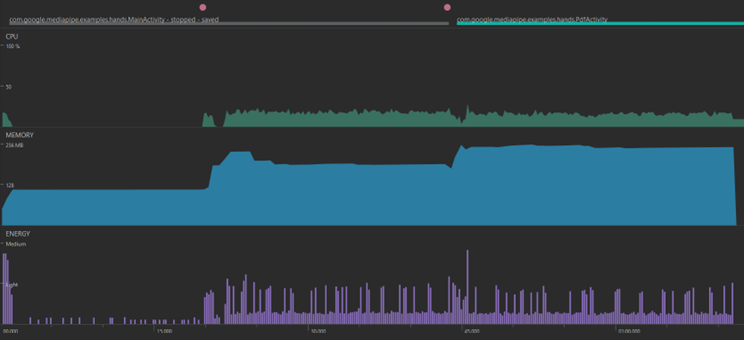
\includegraphics[width=0.8\textwidth]{images/profiling_app.png}
\end{figure}

\noindent Il profiling è suddiviso in tre sezioni che corrispondono alle tre pagine visualizzabili, in ordine: pagina \texttt{home}, pagina \texttt{start camera} e pagina \texttt{PdfReader}.\\
Nel complesso non abbiamo misurazioni stravolgenti, la CPU viene utilizzata mediamente il 17\% del suo potenziale quando il tracking delle mani è attivato (\texttt{start camera} e \texttt{PdfReader}), mentre nella \texttt{home} page, dove non succede nulla, giustamente il consumo è nullo tranne che al suo primo caricamento.\\
La memoria viene utilizzata principalmente nella gestione dei Pdf con picchi massimi di 256MB.\\
\\
\noindent Sotto il punto di vista dei consumi Android Studio pone nell'asse delle ordinate tre livelli: Light, Medium e High.\\
Al di là dei cambi di pagina che vengono etichettati come Medium, il consumo generale viene considerato Light.\\
Siccome questo dato non ci ha orientato più di tanto per capire se tale consumo possa essere considerato tollerabile, come accennato in precedenza, abbiamo provato molto empiricamente a verificare di quanto scendeva il livello di batteria durante l'utilizzo dell'app, realizzando un calo di un 2\% ogni 4 minuti con una batteria 4000mAh.\\
Facendo lo stesso con la nota app \textit{Instagram} il consumo è risultato differente, con un uso di un 2\% ogni 7 minuti; quindi messa a confronto la nostra applicazione consuma il doppio.\\
\\
\noindent Ipotizzando uno scenario realistico dove consideriamo il 100\% di batteria di un utente intenzionato a studiare con la nostra applicazione (con le specifiche di dispositivo citate prima) e dedicando un 80\% alla nostra applicazione si ottiene una durata massima di 2 ore e mezza.\\
Esito non troppo deludente, ma pensare che dopo 2 ore e mezza di lettura il dispositivo diviene inutilizzabile non è molto invitante. La situazione si potrebbe però invertire se si cambia il contesto in cui si utilizza il riconoscimento gesture.



\section{Opinioni e sviluppi futuri}
La possibilità di poter interagire con un dispositivo tramite una videocamera introduce un metodo alternativo di interazione con la macchina. Nel corso degli anni i computer si sono evoluti sempre di più mentre il metodo per interagire con essi è rimasto sempre lo stesso: tastiera e mouse.\\
Solo nell'ultimo decennio, grazie ad una sufficiente maturazione della tecnologia, si è cominciato concretamente a implementare mezzi differenti per comunicare con i dispositivi. D'altronde siamo di fronte ad una situazione dove due macchine computazionali potenti (cervello e computer) sono ostacolate, nella loro collaborazione, dalle limitazioni imposte dai metodi tradizionali di interazione ed è per questo che nuove soluzioni che rendono più immediato e naturale il controllo di dispositivi elettronici diventeranno sempre più rilevanti negli anni a seguire.\\
\\
\noindent Il nostro team si è occupato di analizzare un “proof-of-concept” di una applicazione PdfReader gestita non dall'interazione offerta dallo schermo touch ma dalla videocamera frontale che rileva specifiche gesture. Svolgendo i test finali siamo rimasti soddisfatti del risultato; l'unico tallone d'Achille risiede nelle limitazioni imposte dai modelli di riconoscimento.
Esistono diversi metodi che potrebbero aiutare a migliorare i risultati del modello ML, come ad esempio software in grado di incorporare dati ricevuti da sensori LiDAR a immagini ricevute da una videocamera, come modelli più recenti di iPhone©, in modo da fornire ai modelli ML informazioni sulla distanza della scena ripresa.\\
\\
\noindent In questo progetto ci si è limitati alla gestione di un pdf, ma una volta che la logica di gesture detection è stata messa a punto e anche il consumo migliorato, cambiare scenario diviene immediato: è sufficiente collegare le gesture a determinate azioni. Un esempio potrebbe essere la simulazione del cursore tramite gesture, permettendo quindi di navigare nell'interfaccia proposta dallo schermo. Combinando poi il \\
riconoscimento delle mani con altri tipi di riconoscimenti (face, body, ...) potrebbe nascere qualcosa di interessante. Rimanendo però nel mondo mobile, dove le risorse energetiche e computazionali sono preziose e limitate, il framerate relativamente contenuto non permette di riconoscere accuratamente gesture dinamiche veloci, ciò nonostante si riescono a realizzare applicazioni con interazioni più naturali rispetto ai classici pulsanti.


\epigraph{It was the stylus. I killed the Newton because of the stylus, if you're holding it, you can't use the other five that are attached to your wrist.}{Steve Jobs Movie, 2015}
